\documentclass{article}
%\usepackage[spanish]{babel} 
%\selectlanguage{english}  
\usepackage[utf8]{inputenc} 
\usepackage[T1]{fontenc} 
\usepackage{array}
\usepackage{geometry}
 \geometry{
 a4paper,
 total={170mm,257mm},
 left=20mm,
 top=20mm,
 }
\usepackage{amsmath, amsthm, amsfonts} 
\usepackage{graphicx} 
\usepackage[colorinlistoftodos]{todonotes} 
\usepackage[colorlinks=true, allcolors=blue]{hyperref} 
\usepackage[square,numbers]{natbib}
\usepackage{upgreek}
\usepackage{lipsum}  
\usepackage{diagbox}


\title{Informe Proyecto Final Grupo 6}
\author{Benjam\'in Ignacio Ayala Baeza  \\ \href{mailto:beayala2021@udec.cl}{beayala2021@udec.cl} 
        \and Mar\'ia Ignacia Espinoza Inzunza \\ \href{mailto:marespinoza2021@udec.cl}{marespinoza2021@udec.cl} \\
        \and Florencia Andrea Fuentes Jara \\ \href{mailto:flofuentes2021@udec.cl}{flofuentes2021@udec.cl} \\
        \and Mart\'in Andrés Sepúlveda Zu\~niga \\ \href{mailto:msepulveda2021@udec.cl}{msepulveda2021@udec.cl} \\
\date{Universidad de Concepci\'on \\ \today}
}
\setlength{\marginparwidth}{2cm}
\begin{document}
\maketitle

\begin{abstract}

En el presente documento buscamos encontrar la relación entre la distancia de lanzamiento de una fuerza aplicada a un cuerpo circular y el giro que se produce. Esto midiendo el número de giros a distintas distancias del cuerpo y con varias repeticiones para eliminar el error aleatorio. Además de graficamos nuestros datos y realizamos varios ajustes para analizar cuál se asimila más a nuestro modelo esto viéndolo con el análisis de sus respectivos residuos. Para así concluir con alguna correspondencia entre nuestras variables.

\end{abstract}

\section{Introducción} \label{intro}
 A lo largo de este informe expondremos nuestros procedimiento, resultados y análisis para nuestro proyecto de laboratorio del curso Laboratorio I haciendo uso de los conocimientos adquiridos durante el curso.\\
 Nuestra premisa para este experimento consta de estudiar de una manera eficaz los efectos de la aplicación de una fuerza aplicada de manera tangencial a un objeto que posee una capacidad de rotación. 
A partir de este efecto, mostraremos a traves del analisis de datos la tendencia de crecimiento la cantidad de vueltas que medimos en la cinta metrica a partir de la distancia aplicada. Con esta recoleccion de datos haremos uso de los conocimientos adqueridos, haciendo un ajuste de los datos para un mejor y correcto analisis. 




% ESTO NO - JAJA Basaremos nuestro estudio sobre el fenómeno del torque y del momento angular (juntos con su conservación) y como este ultimo principio no es tan efectivo ante las condiciones definidas en la literatura. Tal como veremos en nuestro experimento, notaremos que las condiciones representadas en las ecuaciones y los libros son bastante lejanas a las condiciones que veremos en la practica, esto nos obliga a trabajar con margenes de error, ajustes para los datos de forma que podamos estudiar la tendencia teórica con la practica. 
\section{Objetivos}
Nuestros objetivos a lograr con esta actividad de laboratorio son :

\begin{itemize}
    \item Encontrar la relación entre la distancia de lanzamiento del medidor de una cinta métrica con el número de giros que esta hace en una plataforma en nuestro caso la mesa del laboratorio.
    \item Comparar nuestros resultados con algún hecho cotidiano o fenómeno físico relacionado. %??? nose q chucha sera eso si
\end{itemize}

\section{Marco Teórico}

\section{Experimentación}
Para encontrar la correlación entre distancia y cantidad de vueltas, debemos repetir el experimento en diversas condiciones. Nuestra condición variable corresponde a la distancia desde la cual veremos como afecta la fuerza con la cual la cinta métrica se cierra.

\subsection{Materiales}
En este proyecto utilizamos los siguientes instrumentos:

\begin{itemize}
    \item[-] Cinta Métrica 3 $[\text{m}]$
    \item[-] Papel con ejes de referencia
    \item[-] Cinta adhesiva
    \item[-] Celular con cámara lenta
    \item[-] Mesa
\end{itemize}
    
\subsection{Montaje Experimental}
  En la figura \ref{fig:montaje} mostramos los materiales utilizados para el montaje de nuestro experimento.
  
    \begin{figure}[ht]
        \centering
        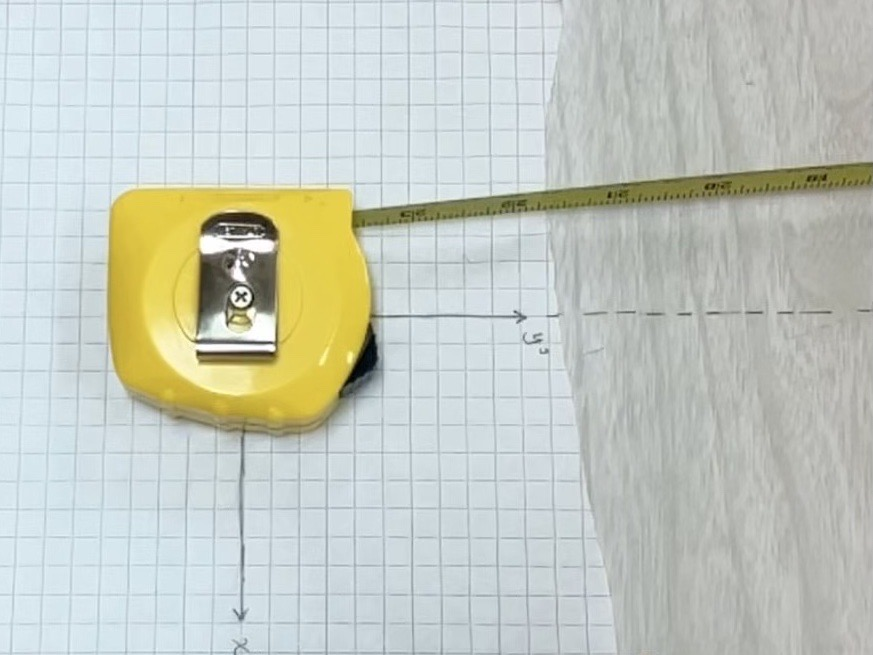
\includegraphics[scale=0.25]{Informe/img/montaje1.png}
        \caption{Fotografía de montaje experimental}
        \label{fig:montaje}
    \end{figure}
    
\subsection{Procedimiento}
A continuación describiremos detalladamente el paso a paso realizado para las diversas mediciones hechas:

\begin{enumerate}
    \item Comenzamos colocando la cinta métrica al centro del papel con ejes de referencia, de forma que si extendemos la cinta métrica esta crece a lo largo del eje de las ordenadas. La cinta métrica y debe estar pegada al papel, esto lo logramos usando la cinta adhesiva.
    \item Alineamos en nuestra mesa el papel con ejes de referencia y proyectamos estos ejes en la mesa, de forma que tengamos una extensión de estos para observar cuanto gira el montaje de la cinta métrica con el papel. 
    \item Posicionamos nuestro celular con cámara lenta por encima del montaje del papel, mesa y cinta de forma que tengamos una visión área del sistema.
    \item Tomamos el comienzo de la cinta métrica y extendemos hasta llegar a los $10 [cm]$, soltamos la cinta y vemos cuanto gira. Todo este proceso mientras grabamos. \label{4} 
    \item Repetimos el paso \ref{4}. diez veces y anotamos los resultados. \footnote{Idealmente recomendamos tomar más repeticiones, ya que entre más repeticiones menos error aleatorio va haber, pero en este proyecto en particular por temas de tiempo tuvimos que dejarlos en diez repeticiones.}
    \item Repetimos todo el procedimiento para la medida de la cinta métrica igual a 20 [cm], 30 [cm], 40 [cm], 50 [cm], 60 [cm], 70 [cm], 80 [cm], 90 [cm] y 100 [cm].
          %falta decir q lo grabamos y q aqui hay fote y video wuajajajaj  
\end{enumerate}

\subsection{Procesamiento de datos}
El procedimiento para la extracción de datos, en este caso el ángulo total de giro, se hizo mediante el post procesamiento de imágenes, primero se analizo si es que   
    


\section{Resultados y Análisis}

%tablitaa
 
\begin{table}[]
\centering
\begin{tabular}{|c|l|l|l|l|l|l|l|l|l|l|}
\hline
 \diagbox[width=8em,trim=lr]{\small{N$^\circ_{rep}$}}{\small{Long tiro}} & 10 \scriptsize{$[cm]$} & 20 \scriptsize{$[cm]$}  & 30 \scriptsize{$[cm]$}  & 40 \scriptsize{$[cm]$}  & 50\scriptsize{$[cm]$}  & 60 \scriptsize{$[cm]$} & 70 \scriptsize{$[cm]$} & 80 \scriptsize{$[cm]$} & 90 \scriptsize{$[cm]$} & 100 \scriptsize{$[cm]$} \\ \hline
1  & $79.0^\circ$ & $182.0^\circ$ & $258.0^\circ$ & $472.0^\circ$ & $400.0^\circ$ & $399.0^\circ$ & $670.0^\circ$ & $547.0^\circ$ & $797.0^\circ$ & $676.0^\circ$   \\ \hline
2  & 69.0 & 175.0 & 253.0 & 448.0 & 450.0 & 383.0 & 587.0 & 688.0 & 599.0 & 691.0  \\ \hline
3  & 87.0 & 190.0 & 254.0 & 454.0 & 400.0 & 524.0 & 516.0 & 740.0 & 646.0 & 640.0  \\ \hline
4  & 76.0 & 193.0 & 290.0 & 455.0 & 550.0 & 509.0 & 458.0 & 765.0 & 698.0 & 683.0  \\ \hline
5  & 61.0 & 186.0 & 343.0 & 409.0 & 349.0 & 613.0 & 432.0 & 541.0 & 584.0 & 761.0  \\ \hline
6  & 42.0 & 201.0 & 255.0 & 334.0 & 354.0 & 608.0 & 532.0 & 666.0 & 763.0 & 713.0  \\ \hline
7  & 48.0 & 214.0 & 234.0 & 321.0 & 580.0 & 485.0 & 407.0 & 675.0 & 580.0 & 729.0  \\ \hline
8  & 75.0 & 175.0 & 214.0 & 305.0 & 490.0 & 550.0 & 561.0 & 441.0 & 508.0 & 811.0  \\ \hline
9  & 25.0 & 220.0 & 263.0 & 268.0 & 520.0 & 495.0 & 461.0 & 612.0 & 501.0 & 549.0  \\ \hline
10 & 74.0 & 202.0 & 297.0 & 242.0 & 300.0 & 389.0 & 465.0 & 538.0 & 540.0 & 575.0  \\ \hline
\end{tabular}
\end{table}


\section{Conclusión}


\bibliographystyle{apalike}
\bibliography{Informe/referencias.bib}
\end{document}